\documentclass[a4paper, 12pt]{book}
%\usepackage[T1]{fontenc}
\usepackage{bera}% optional: just to have a nice mono-spaced font
\usepackage{listings}
\usepackage{xcolor}
\colorlet{punct}{red!60!black}
\definecolor{delim}{RGB}{20,105,176}
\colorlet{numb}{magenta!60!black}
\definecolor{maroon}{cmyk}{0, 0.87, 0.68, 0.32}
\definecolor{halfgray}{gray}{0.55}
\definecolor{ipython_frame}{RGB}{207, 207, 207}
\definecolor{ipython_bg}{RGB}{247, 247, 247}
\definecolor{ipython_red}{RGB}{186, 33, 33}
\definecolor{ipython_green}{RGB}{0, 128, 0}
\definecolor{ipython_cyan}{RGB}{64, 128, 128}
\definecolor{ipython_purple}{RGB}{170, 34, 255}

\lstdefinelanguage{json}{
    stepnumber=1,
   	identifierstyle=\color{black}\ttfamily,
    numbersep=8pt,
    showstringspaces=false,
    breaklines=true,
    backgroundcolor=\color{ipython_bg},
    identifierstyle=\color{black}\ttfamily,
    commentstyle=\color{ipython_cyan}\ttfamily,
    stringstyle=\color{ipython_red}\ttfamily,
    keepspaces=true,
    showspaces=false,
    showstringspaces=false,
    rulecolor=\color{ipython_frame},
    frame=single,
    frameround={t}{t}{t}{t},
    framexleftmargin=5mm,
    numbers=left,
    numberstyle=\tiny\color{halfgray},
    % extendedchars=true,
    basicstyle=\scriptsize,
    keywordstyle=\color{ipython_green}\ttfamily,
    literate=
     *{0}{{{\color{numb}0}}}{1}
      {1}{{{\color{numb}1}}}{1}
      {2}{{{\color{numb}2}}}{1}
      {3}{{{\color{numb}3}}}{1}
      {4}{{{\color{numb}4}}}{1}
      {5}{{{\color{numb}5}}}{1}
      {6}{{{\color{numb}6}}}{1}
      {7}{{{\color{numb}7}}}{1}
      {8}{{{\color{numb}8}}}{1}
      {9}{{{\color{numb}9}}}{1}
      {:}{{{\color{punct}{:}}}}{1}
      {,}{{{\color{punct}{,}}}}{1}
      {\{}{{{\color{delim}{\{}}}}{1}
      {\}}{{{\color{delim}{\}}}}}{1}
      {[}{{{\color{delim}{[}}}}{1}
      {]}{{{\color{delim}{]}}}}{1},
}




\lstset{
    breaklines=true,
    extendedchars=true,
    literate=
    {á}{{\'a}}1 {é}{{\'e}}1 {í}{{\'i}}1 {ó}{{\'o}}1 {ú}{{\'u}}1
    {Á}{{\'A}}1 {É}{{\'E}}1 {Í}{{\'I}}1 {Ó}{{\'O}}1 {Ú}{{\'U}}1
    {à}{{\`a}}1 {è}{{\`e}}1 {ì}{{\`i}}1 {ò}{{\`o}}1 {ù}{{\`u}}1
    {À}{{\`A}}1 {È}{{\'E}}1 {Ì}{{\`I}}1 {Ò}{{\`O}}1 {Ù}{{\`U}}1
    {ä}{{\"a}}1 {ë}{{\"e}}1 {ï}{{\"i}}1 {ö}{{\"o}}1 {ü}{{\"u}}1
    {Ä}{{\"A}}1 {Ë}{{\"E}}1 {Ï}{{\"I}}1 {Ö}{{\"O}}1 {Ü}{{\"U}}1
    {â}{{\^a}}1 {ê}{{\^e}}1 {î}{{\^i}}1 {ô}{{\^o}}1 {û}{{\^u}}1
    {Â}{{\^A}}1 {Ê}{{\^E}}1 {Î}{{\^I}}1 {Ô}{{\^O}}1 {Û}{{\^U}}1
    {œ}{{\oe}}1 {Œ}{{\OE}}1 {æ}{{\ae}}1 {Æ}{{\AE}}1 {ß}{{\ss}}1
    {ç}{{\c c}}1 {Ç}{{\c C}}1 {ø}{{\o}}1 {å}{{\r a}}1 {Å}{{\r A}}1
    {€}{{\EUR}}1 {£}{{\pounds}}1
}

\lstdefinelanguage{python}{
    morekeywords={access,and,break,class,continue,def,del,elif,else,except,exec,finally,for,from,global,if,import,in,is,lambda,not,or,pass,print,raise,return,try,while},
    morekeywords=[2]{abs,all,any,basestring,bin,bool,bytearray,callable,chr,classmethod,cmp,compile,complex,delattr,dict,dir,divmod,enumerate,eval,execfile,file,filter,float,format,frozenset,getattr,globals,hasattr,hash,help,hex,id,input,int,isinstance,issubclass,iter,len,list,locals,long,map,max,memoryview,min,next,object,oct,open,ord,pow,property,range,raw_input,reduce,reload,repr,reversed,round,set,setattr,slice,sorted,staticmethod,str,sum,super,tuple,type,unichr,unicode,vars,xrange,zip,apply,buffer,coerce,intern},
    sensitive=true,
    morecomment=[l]\#,
    morestring=[b]',
    morestring=[b]",
    morestring=[s]{'''}{'''},
    morestring=[s]{"""}{"""},
    morestring=[s]{r'}{'},
    morestring=[s]{r"}{"},
    morestring=[s]{r'''}{'''},
    morestring=[s]{r"""}{"""},
    morestring=[s]{u'}{'},
    morestring=[s]{u"}{"},
    morestring=[s]{u'''}{'''},
    morestring=[s]{u"""}{"""},
    % {replace}{replacement}{lenght of replace}
    % *{-}{-}{1} will not replace in comments and so on
    literate=
    {á}{{\'a}}1 {é}{{\'e}}1 {í}{{\'i}}1 {ó}{{\'o}}1 {ú}{{\'u}}1
    {Á}{{\'A}}1 {É}{{\'E}}1 {Í}{{\'I}}1 {Ó}{{\'O}}1 {Ú}{{\'U}}1
    {à}{{\`a}}1 {è}{{\`e}}1 {ì}{{\`i}}1 {ò}{{\`o}}1 {ù}{{\`u}}1
    {À}{{\`A}}1 {È}{{\'E}}1 {Ì}{{\`I}}1 {Ò}{{\`O}}1 {Ù}{{\`U}}1
    {ä}{{\"a}}1 {ë}{{\"e}}1 {ï}{{\"i}}1 {ö}{{\"o}}1 {ü}{{\"u}}1
    {Ä}{{\"A}}1 {Ë}{{\"E}}1 {Ï}{{\"I}}1 {Ö}{{\"O}}1 {Ü}{{\"U}}1
    {â}{{\^a}}1 {ê}{{\^e}}1 {î}{{\^i}}1 {ô}{{\^o}}1 {û}{{\^u}}1
    {Â}{{\^A}}1 {Ê}{{\^E}}1 {Î}{{\^I}}1 {Ô}{{\^O}}1 {Û}{{\^U}}1
    {œ}{{\oe}}1 {Œ}{{\OE}}1 {æ}{{\ae}}1 {Æ}{{\AE}}1 {ß}{{\ss}}1
    {ç}{{\c c}}1 {Ç}{{\c C}}1 {ø}{{\o}}1 {å}{{\r a}}1 {Å}{{\r A}}1
    {€}{{\EUR}}1 {£}{{\pounds}}1
    %
    {^}{{{\color{ipython_purple}\^{}}}}1
    {=}{{{\color{ipython_purple}=}}}1
    %
    {+}{{{\color{ipython_purple}+}}}1
    {*}{{{\color{ipython_purple}$^\ast$}}}1
    {/}{{{\color{ipython_purple}/}}}1
    %
    {+=}{{{+=}}}1
    {-=}{{{-=}}}1
    {*=}{{{$^\ast$=}}}1
    {/=}{{{/=}}}1,
    literate=
    *{-}{{{\color{ipython_purple}-}}}1
     {?}{{{\color{ipython_purple}?}}}1,
    %
    identifierstyle=\color{black}\ttfamily,
    commentstyle=\color{ipython_cyan}\ttfamily,
    stringstyle=\color{ipython_red}\ttfamily,
    keepspaces=true,
    showspaces=false,
    showstringspaces=false,
    rulecolor=\color{ipython_frame},
    frame=single,
    frameround={t}{t}{t}{t},
    framexleftmargin=5mm,
    numbers=left,
    numberstyle=\tiny\color{halfgray},
    backgroundcolor=\color{ipython_bg},
    % extendedchars=true,
    basicstyle=\scriptsize,
    keywordstyle=\color{ipython_green}\ttfamily,
}
\usepackage[a4paper, left=2.5cm, right=2.5cm, top=3cm, bottom=3cm]{geometry}
\usepackage{times}
\usepackage[utf8]{inputenc}
\usepackage[spanish]{babel} % Comenta esta línea si tu memoria es en inglés
\usepackage{url}
%\usepackage[dvipdfm]{graphicx}
\usepackage{graphicx}
\usepackage{float}  %% H para posicionar figuras
\usepackage[nottoc, notlot, notlof, notindex]{tocbibind} %% Opciones de índice
\usepackage{latexsym}  %% Logo LaTeX
\usepackage{enumitem}

\title{Memoria del Proyecto}
\author{Santiago Carrión Vivanco}

\renewcommand{\baselinestretch}{1.5}  %% Interlineado

\begin{document}

\renewcommand{\refname}{Bibliografía}  %% Renombrando
\renewcommand{\appendixname}{Apéndice}

%%%%%%%%%%%%%%%%%%%%%%%%%%%%%%%%%%%%%%%%%%%%%%%%%%%%%%%%%%%%%%%%%%%%%%%%%%%%%%%%
% PORTADA

\begin{titlepage}
\begin{center}
\begin{tabular}[c]{c c}
%\includegraphics[bb=0 0 194 352, scale=0.25]{logo} &

\includegraphics[scale=0.25]{img/urjc_logo.jpg} &
\begin{tabular}[b]{l}
\Huge
\textsf{UNIVERSIDAD} \\
\Huge
\textsf{REY JUAN CARLOS} \\
\end{tabular}
\\
\end{tabular}

\vspace{3cm}

\Large
GRADO EN INGENIERÍA TELEMÁTICA

\vspace{0.4cm}

\large
Curso Académico 2017/2018

\vspace{0.8cm}

Trabajo Fin de Grado

\vspace{2.5cm}

\LARGE
SCRATCH4ROBOTS

\vspace{4cm}

\large
Autor : Santiago Carrión Vivanco \\
Tutor : Jose María Cañas Plaza
\end{center}
\end{titlepage}

\newpage
\mbox{}
\thispagestyle{empty} % para que no se numere esta pagina

\maketitle

\cleardoublepage
% Las buenas noticias es que los \'indices se generan autom\'aticamente.
% Lo \'unico que tienes que hacer es elegir cu\'ales quieren que se generen,
% y comentar/descomentar esa instrucci\'on de LaTeX.

%%%% \'indice de contenidos
\tableofcontents 
%%%% \'indice de figuras
\cleardoublepage
%\addcontentsline{toc}{chapter}{Lista de figuras} % para que aparezca en el indice de contenidos
\listoffigures % indice de figuras
%%%% \'indice de tablas
%\cleardoublepage
%\addcontentsline{toc}{chapter}{Lista de tablas} % para que aparezca en el indice de contenidos
%\listoftables % indice de tablas

\cleardoublepage
\pagestyle{plain}
\pagenumbering{arabic}
\chapter{Introducción}
\section{Robótica}
\label{sec:robotica}

La palabra Robot se deriva de la palabra de origen checoslovaco robota, que quiere decir siervo. Dicha palabra apareció por primera vez en la literatura en la obra R.U.R (1921)(Robot Universalis de Rossum), de Karel Capek.

Un robot es un sistema electromecánico que utiliza una serie de elementos hardware
(actuadores, sensores y procesadores) y cuyo comportamiento viene controlado por un
software programable que le da la inteligencia. La robótica se puede ver como la ciencia
y la tecnología de los robots, donde se combinan varias disciplinas como la mecánica, la
informática, la electrónica y la ingeniería artificial, que hacen posible el diseño hardware y software del robot.

Los robots se componen esencialmente de tres tipos de dispositivos: sensores,
procesadores y actuadores. En un robot los sensores son los encargados de recoger
la información del entorno. En este grupo se situarían: el láser, el sonar o las
cámaras. Estos dispositivos equivaldrían a nuestros sentidos humanos. Por otro lado se
encuentran los procesadores, encargados de analizar los datos que le son suministrados
por los sensores, también son los encargados de elaborar una respuesta a estos datos y
enviar la acción que deba llevarse a cabo a los actuadores, son como nuestro cerebro.
Por último los actuadores, principalmente motores eléctricos, se encargan de interactuar
con el entorno del mismo modo que lo hacen nuestros músculos.


\subsection{Historia}
\label{subsec:historia}
A finales del siglo XIX se presentan las primeras máquinas \textit{robots}, pero no
será hasta la segunda guerra mundial cuando se realicen los primeros diseños de esta
naturaleza.Con el desarrollo de las primeras computadoras digitales se produjo una
considerable evolución en este campo. Así, en 1970 una serie de investigadores del
Instituto de Investigación de Stanford desarrollaron Shakey (figura 1.1). Su sistema de
control creaba una reproducción interna del entorno a partir de los sensores de que
disponía y desde ella calculaba su movimiento.

Aunque es un termino relativamente nuevo y cuyo uso extendido es muy reciente, la historia lleva siglos dando pasos para llegar al punto en el que nos encontramos.
Durante la época de los griegos se intentó crear dispositivos que tuvieran un movimiento sin fin, que no fuera controlado ni supervisado por personas, en los siglos XVII y XVIII la construcción de autómatas humanoides fabricados con mecanismos de relojería por Jacques de Vaucanson, Pierre Henri-Louis, Jaquet- Droz, como el escribiente, the Draughtsman, el músico Henri Maillar det (1800), Olimpia de la ópera de Offenback de Hoffman, fortalecieron la búsqueda de mecanismos que auxiliaran a los hombres en sus tareas.

Es En 1926  con \textit{Metrópolis} , de Fritz Lang, la primera película en la que aparecen robots cuando se empieza a dar a conocer el termino de forma popular.
En 1950 Isaac Asimov publica el libro \textit{Yo Robot}, con las tres leyes de la robótica:

\textit{Un robot no puede lastimar a un ser humano o permanecer inactivo ante un daño que se le pueda hacer.}

\textit{El robot debe obedecer al ser humano excepto si contradice la primera ley.}

\textit{El robot debe proteger su existencia salvo que entre en conflicto con las leyes anteriores.}

Gracias a este libro, Isaac Asimov hizo popular la robótica.
Durante la Segunda Guerra Mundial aparecieron gran variedad de
mecanismos de control y pilotaje automático, también máquinas cibernéticas, donde los robots empezaban a perder su forma humana, llegando a la actualidad con la pérdida total de su antropomorfismo debido a que se concibe a los robots según su función.
Pero sin duda uno de los mayores impulsos en este mundo se produce con la llegada de la industrialización masiva. A principios de los 60, se instaló en una cadena de General Motors el primer robot industrial, Unimate \ref{fig:unimate}, que realizaba tareas en la cadena de producción de los vehículos que podían ser peligrosas para los trabajadores.

En la misma década se creó el robot Shakey, el primero que combinó razonamiento lógico con acción física \ref{fig:shakey}. Al igual que en el caso que trata este trabajo, Shakey utilizaba Planificación Automática para determinar sus acciones.

\begin{figure}[!htb]
	\begin{minipage}{0.48\textwidth}
    	\centering
     	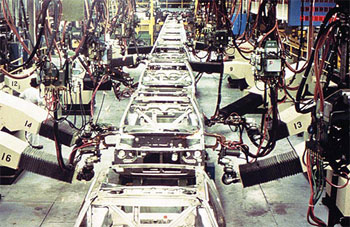
\includegraphics[scale=0.5]{img/unimate.jpg}
  		\caption{Unimate, General Motors}
  		\label{fig:unimate}
   	\end{minipage}\hfill
   	\begin {minipage}{0.48\textwidth}
     	\centering
     	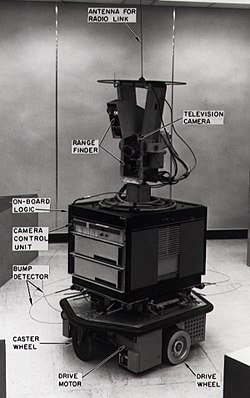
\includegraphics[scale=0.5]{img/shakey.jpg}
     	\caption{shakey en 1972}
     	\label{fig:shakey}
	\end{minipage}
\end{figure}

En 1970 se continua con la dinámica de crecimiento del sector, debido esta vez a la evolución del software ocurrida en esta época, y no parará hasta nuestros días, teniendo un crecimiento exponencial con una fuerte correlación con la evolución de software y hardware en general.
Desde este momento todas las grandes empresas dotaran sus fábricas de robots industriales. 

No es hasta 1996 cuando la empresa japonesa Honda presentó el robot P2, robot bípedo con forma humana que era capaz de caminar, empujar objetos, subir o bajar escaleras.
En la actualidad uno de los mayores logros en el mundo de la robótica se da en 2011, la NASA lanzó al espacio el robot tipo vehículo explorador \textit{Curiosity} \ref{fig:curiosity} , que aterrizó en Marte al año siguiente. Su principal cometido es investigar la capacidad pasada y presente del planeta para alojar vida.

\begin{figure}[!ht]
    \centering
    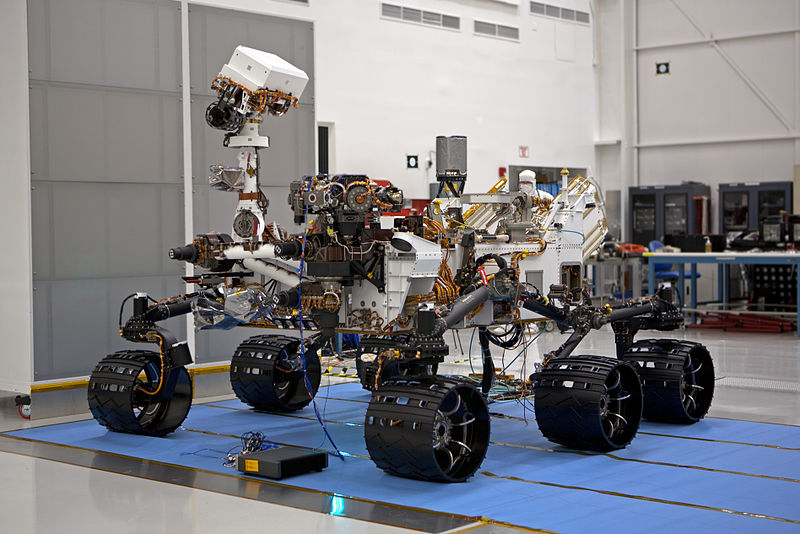
\includegraphics[scale=0.75]{img/curiosity.jpg}
  	\caption{El Curiosity en el Laboratorio de Propulsión a Chorro de la NASA}
  	\label{fig:curiosity}
\end{figure}

\subsection{Diferentes aplicaciones}
\label{subsec:diferentes aplicaciones}

Actualmente la robótica se encuentra en muchos ambitos de nuestra vida cotidiana, algunas aplicaciones son:

La \textbf{robótica educativa} o robótica pedagógica es una disciplina que trabaja en la concepción creación e implementación de prototipos robóticos y programas con fines pedagógicos. Con ello se permite al alumno fabricar sus representaciones sobre los fenómenos del mundo, facilitar su adquisición y trasferencia a distintas áreas de conocimiento.
A través de la robótica educativa, los docentes pueden desarrollar de una forma práctica los conceptos teóricos que suelen ser abstractos y confusos, además despierta el interés del alumno por esos temas y relaciona al niño con el mundo tecnológico en el que se mueve. El empleo de un ambiente de aprendizaje basado en la robótica educativa ayuda al desarrollo de nuevas habilidades y conceptos, fortalece el pensamiento lógico, estructurado y formal del alumnado, desarrollando su capacidad para resolver problemas concretos.
Una de las características de este ámbito es la capacidad que posee para mantener la
atención del alumno, ya que manipula y experimenta haciendo que se concentre en sus
percepciones y observaciones sobre la actividad que realiza. Actualmente existen varios kits de robótica, algunos de ellos son: LEGO MINDSTORMS education, LEGO WeDo, LEGO NXT o Parallax Scribbler. Además, también existe la posibilidad de trabajar con programas con los que controlar y simular diferentes La robótica en Educación Infantil. Realidades y limitaciones robots como son NXT-G Educación, ROBOTC, ROBOLAB o Microsoft Robotics Developer Studio.

La \textbf{robótica en la medicina}, involucra en si varios ámbitos ya sea en cirugías de alto riesgo, en rehabilitaciones, en ayuda a personas con enfermedades de movilidad o discapacitados, en el almacenamiento de medicamentos y también en lo que se trata en pruebas ficticias y cirugías computarizadas.

En el ámbito \textbf{militar}, la robótica donde más ha evolucionado es en la creación de vehiculos autónomos, tecnología que tras unos años pasa a a ser de uso civil.
Algunas de las creaciones que nos hemos heredados es el UAV, que se conocen comúnmente como dron, es una aeronave que vuela sin tripulación, Capaz de mantener de manera autónoma un nivel de vuelo controlado y sostenido, y propulsado por un motor de explosión, eléctrico, o de reacción.

\textbf{Robotica aeroespacial}: Uno de los mayores impulsores de la robótica ha sido la conquista del espacio, esta es una parte fundamental de la exploración espacial, debido a la imposibilidad de ser realizada en primera mano por un humano.
La idea básica sobre Robots Espaciales consiste en utilizar Inteligencia Artificial para
permitir a los robots realizar labores de exploración como si de un humano se tratase, desplazarse en terrenos y ambientes complejos de forma autónoma sin más conocimiento que lo recibido por sus sensores. Se busca no solo el proceso de pensamiento y análisis de los humanos en determinar las características del terreno, sino también la habilidad humana de conducir un vehículo en tiempo real.

-INDUSTRIAL
-AUTOMOVILISMO

\subsection{Tipos de Robots}
\label{subsec:tipos de robots}

Ningún autor se pone de acuerdo en cuántos y cuáles son los tipos de robots y sus características esenciales. La más común son la que a continuación se presentan:

\textbf{Segun su Estructura}:
\begin{description}[align=left]
\item [Androides]: estos artilugios se parecen y actúan como si fueran seres humanos. Este tipo de robots no existen en la realidad, por lo menos por el momento, sino que son elementos ficcionales.

\item [Poliarticulados]: En este grupo pueden encontrarse robots de diversas formas y configuraciones, pero su característica en común es la de ser sedentarios. Es decir, que son robots estructurados para moverse en un determinado espacio de trabajo, según uno o más sistemas de coordenadas y con un número limitado de grados de libertad.

\item [Móviles]: estos robots cuentan con orugas, ruedas o patas que les permiten desplazarse de acuerdo a la programación a la que fueron sometidos. Estos robots cuentan con sistemas de sensores, que son los que captan la información que dichos robots elaboran. Los móviles son utilizados en instalaciones industriales, en la mayoría de los casos para transportar la mercadería en cadenas de producción así como también en almacenes. Además, son herramientas muy útiles para investigar zonas muy distantes o difíciles de acceder, es por eso que en se los utiliza para realizar exploraciones espaciales o submarinas.

\item [Zoomórficos]: la locomoción de estos robots imita a la de distintos animales y se los puede dividir en caminadores y no caminadores. Estos últimos están aún muy poco desarrollados mientras que los caminadores sí lo están y resultan útiles para la exploración volcánica y espacial.

\item [Híbridos]: Este término corresponde a todos aquellos robots que son difíciles de clasificar, ya que corresponden a una combinación de las estructuras anteriormente explicadas. Por ejemplo, un robot híbrido, que esté conformado por la segmentación de articulaciones y ruedas, podría ser considerado tanto móvil, así como zoomórfico.
\end{description}

\textbf{Segun su Cronologia}:
\begin{description}[align=left]
\item [1ª Generación. Manipuladores]: Son sistemas mecánicos multifuncionales con un sencillo sistema de control, bien manual, de secuencia fija o de secuencia variable.

\item [2ª Generación. Robots de aprendizaje]: Repiten una secuencia de movimientos de movimientos que ha sido ejecutada previamene por un operador humano. El modo de hacerlo es a través de un dispositivo mecánico. El operador realiza los movimientos requeridos mientras el robot le sigue y los memoriza.

\item [3ª Generación. Robots con control sensorizado]: El controlador es una computadora que ejecuta las órdenes de un programa y las envía al manipulador para que realice los movimientos necesarios.

\item [4ª Generación. Robots inteligentes]: Son similares a los anteriores, pero además poseen sensores que envían información a la computadora de control sobre el estado del proceso. Esto permite una toma inteligente de decisiones y el control del proceso en tiempo real.
\end{description}

ROBOTICA EN MI TFG


\section{Lenguajes de programación visual}
\label{sec:lenguajes}

Un lenguaje de programación visual es cualquier lenguaje de programación que permite a los usuarios crear programas manipulando elementos del programa gráficamente en lugar de especificarlos textualmente. Permite la programación con expresiones visuales, arreglos espaciales de texto y símbolos gráficos, utilizados como elementos de sintaxis o notación secundaria. Por ejemplo, muchos se basan en la idea de "cajas y flechas", donde las cajas u otros objetos de pantalla se tratan como entidades, conectadas por flechas, líneas o arcos que representan relaciones, mientras que otros se basan en el apilamiento de "cajas" con una funcion predefinida, creando así varios flujos de acciones programáticas con una objetivo final.

Estos lenaguajes por regla general se usan en programación dirigida por eventos, La programación dirigida por eventos es un paradigma de programación en el que el flujo del programa está determinado por eventos o mensajes desde otros programas o hilos de ejecución.
Las aplicaciones desarrolladas con programación dirigida por eventos implementan un bucle principal o main loop donde se ejecutan las dos secciones principales de la aplicación: El selector de eventos y el manejador de eventos.
HISTORIA

Podemos diferenciar varios niveles dentro de los lenguajes de programación visual:

\textbf{Sintaxis}: en el nivel sintáctico, la explicación del bloque está limitada a
estructura del lenguaje. Por ejemplo, una explicación podría revelar que una condición es parte de una declaración IF y no debe ser confundido con una acción que se puede ejecutar en THEN o ELSE parte de una declaración. Sin embargo, este no trata de definir de forma específica qué es lo que define esa condición.
Intentan reducir o incluso eliminar por completo los errores sintácticos y ayudan a la creación de programas bien formados. Una analogía sería el corrector ortográfico en procesadores de texto que subraya o incluso corrige automáticamente palabras o gramática individuales.	

\textbf{Semántica}: en el nivel de la semántica,se dan explicaciones sobre los bloques, a menudo implementadas a través de funciones de ayuda que describen el significado
de un bloque. El usuario obtiene una respuesta semántica en forma de panel de ayuda genérico incluyendo una breve descripción del significado del comando o bloque y la lista de opciones adicionales.

\textbf{Pragmática}: permiten llevar nuestra implementación a un punto de testeo específico, nos ayudan con una serie de modulos propios a crear el entorno necesario para simular el funcionamiento de nuestro programa en ese estado.

\subsection{Motivación}
\label{subsec:motivacion}
Las principales motivaciones del uso de estos lenguajes son su \textbf{accesibilidad}, ya que no requiere de una infraestructura potente para su funcionamiento.
Además el \textbf{facil aprendizaje} hace que sea un lenguaje idoneo para aquellos que no tienen ningún conocimiento de informática previo.
Y por último el eliminar de la ecuación algo tan simple como los \textbf{errores de sintaxis}, nos olvidamos completamente de este tipo de fallos, haciendo el desarrollo más fluido y menos frustrante para los principiantes, algo que puede marcar la diferencia a la hora de encontrar gratificante el desarrollo de aplicaciones con estos lenguajes.

\subsection{Tipos}
\label{subsec:tipos}
\begin{description}
\item[Blocly]: El desarrollo de Blockly comenzó en el verano de 2011, y el primer lanzamiento público fue en Maker Faire en mayo de 2012. Blockly fue originalmente diseñado como un reemplazo para OpenBlocks en App Inventor. [3] Neil Fraser comenzó el proyecto con Quynh Neutron, Ellen Spertus y Mark Friedman como colaboradores.
Es un proyecto de Google y es de código abierto bajo la licencia Apache 2.0. [1] Por lo general, se ejecuta en un navegador web y se asemeja visualmente a Scratch. Blockly también se está implementando para Android e iOS; no todas las funciones basadas en el navegador web están disponibles para Android / iOS.
Blockly utiliza bloques visuales que se unen entre sí para facilitar la escritura de códigos y generar código JavaScript, Python, PHP o Dart. También se puede personalizar para generar código en cualquier lenguaje de computadora textual.

\item[Scratch]:es un proyecto del Grupo Lifelong Kindergarten del MIT Media Lab.
Es utilizado por estudiantes y docentes de todo el mundo para expresar ideas mediante animaciones, juegos e interacciones facilmente programables con este entorno, hablaremos en capitulos siguientes.

\item[Snap!] :desarrollada por la Universidad de California en Berkeley, que sigue la filosofía de facilidad y sencillez para aprender a programar,  Snap se basa en el conocido programa de Scratch, siendo su uso más extendido entre edades más maduras que las de Scratch.
Snap está programado en JavaScript. Esto hace que podamos usarlo desde cualquier navegador, ya sea desde un ordenador como desde las tablets.
En las versiones actuales de Scratch (1.4 ó 2.0) se requiere el uso del plugin privativo de flash player. Si bien es cierto que a partir de la próxima versión 3.0 estará desarrollado íntegramente en HTML5 para que pueda funcionar en la mayoría de dispositivos móviles y tablets. Puedes acceder a este enlace para más información.

\item[Kodu]: originalmente llamado Boku, es un entorno de desarrollo integrado de programación (IDE) de los laboratorios FUSE de Microsoft. Se ejecuta en Xbox 360 y Microsoft Windows XP, Windows Vista, Windows 7, Windows 8 y Windows 10. Fue lanzado en el Xbox Live Marketplace el 30 de junio de 2009. Una versión de Windows está disponible para el público en general para su descarga desde el portal web FUSE de Microsoft. 

\end{description}

\cleardoublepage
\chapter{Objetivos}
Tras haber expuesto las motivaciones y el contexto en el que se engloba este proyecto de fin de grado, en este capítulo daremos una explicación más detallada del problema que se
intenta resolver y los pasos dados para conseguirlo.


\section{Descripción del problema}
\label{sec:descripcion del problema}

En la actualidad la robótoca está en nuestro alrededor en todo momento, debido a las nuevas tecnologías y al abaratamiento de costes se encuentra en plen auge. A pesar de que convivimos a diario con ella por lo general sigue siendo un enigma para la mayoría de las personas.

No es menos cierto que existe una enorme complejidad que requiere de un alto conocimiento de las tecnoligías implicadas tras la configuración de un robot, y es esta barrera la que queremos eliminar.

Con este proyecto buscamos el acercamiento de la robótica a un público con escasos conocimientos técnicos, simplificando al máximo toda la complejidad que existe tras la programación de un robot, hasta el punto que sea usada por niños para el aprendizaje, haciendo el mundo de la robótica más cercano y más atractivo a ojos de aquellos que serán el futuro de ésta.

Esto lo conseguimos creando un nexo entre un lenguaje de programación visual mediante bloques, para esto hacemos uso de \textit{Scratch}, y la programación de robots en Python. Con \textit{Scratch4Robots} conseguimos que partiendo de un lenguaje fácil e intuitivo, basado en el apilamiento de bloques funcionales de código, la traducción a código Python completamente funcional. Creando unos bloques con funcionalidad diriguida a robots en especifico conseguimos que esta traducción pueda ser aplicada a robots.    

\section{Requisitos}
\label{sec:requisitos}

Para cumplir los objetivos marcados de forma satisfactoria, debemos además satisfacer
los siguientes requisitos:

\begin{itemize}
\item El desarrollo deberá ser autocontenido en lo que sea posible, esto quiere decir que todas las librerías y dependencias de nuestra herramienta deberán estar contenidas en su interior. La programación se realizará en el
lenguaje Python.
\item El software desarrollado debrá ser compatible con Ubuntu 16.04, ROS-kinetic y Scratch 2.0 serán los únicos elementos indispensables para el correcto funcionamiento de nuestra herramienta.
\item Todos los componentes desarrollados deberán ser compatibles tanto trabajando en entornos simulados, como usando robots reales, esto se consigue usando todas las abstracciones de las que nos provee JdeRobots, totalmente testadas en robots reales.
\end{itemize}



\section{Metdología de trabajo}
\label{sec:metodologia}

Metodología

\section{Plan de trabajo}
\label{sec:plan}

Simplificaremos la labor a desarrollar en varios puntos:
\begin{itemize}
\item Familiarización con el entorno software: JdeRobot es la plataforma de desarrollo principal utilizada en la mayoría de proyectos realizados en el departamento de robótica
de la URJC. El objetivo principal de esta fase es aprender a utilizar este software, sus
componentes y sus drivers para más adelante utilizarlos como parte de nuestro proyecto.
Como parte del aprendizaje, se desarrolla una herramienta externa al core principal pero que usa de librerías y recurosos de ella.
\item Estudio de KURT: Librería que nos permite obtener toda la información necesaria de un proyecto Scratch, conocimiento de su API y su funcionamiento interno para saber qué podemos llegar a obtener y como usar esa información para proporcionar una traducción robusta al lenguaje Python.
\item Desarrollo de funcionalidades: Aumentamos el número de bloques robóticos própios que podremos usar en Scratch, esto es desarrollar la lógica detras de cada bloque, todo programado en python y la integración de estos bloques con Scratch. Dividimos los bloques entre aptos para drones y robots con ruedas. Estos bloques deben tener una funcionalidad muy específica y funcionar en armonia con el resto, tanto los propios de la aplicación Scratch como los nuevos bloques generados por nosotros propios de aplicaciones robóticas.
\item Facilitar el uso de la herramienta: Haciendo el uso de la herramienta lo más intuitiva posible, mejorando scripts de lanzamiento y de generación de código. Creando ejemplos autocontenidos para una rapida demostración de la potencia de la herramienta. Generando tutoriales tanto escritos como con video para evitar confusiones.
\item Integración: La parte sin duda más compleja del desarrollo ya que se busca que nuestra aplicación sea facilmente instalable en cualquier entorno y con la mayor facilidad posible, únicamente necesitando las dependencias que hemos comentado con anterioridad. Teniendo en cuenta que debe ser facilmente usada por personas con pocos conocimientos técnicos.


\end{itemize}


\cleardoublepage
\chapter{Infraestructura}
\section{Scratch 2.0}
\label{sec:scratch}

Scratch es un proyecto del Grupo Lifelong Kindergarten del MIT Media Lab.
Es utilizado por estudiantes y docentes de todo el mundo para expresar ideas mediante animaciones, juegos e interacciones facilmente programables con este entorno.

El nombre proviene de la palbra \textit{scratching} que en el mundo de la informática se refiere a reutilizar código, el cual puede ser usado de forma beneficiosa y efectiva para otros propósitos y fácilmente combinado, compartido y adaptado a nuevos escenarios, lo cual es una característica clave de Scratch.

Es la segunda versión principal actual de Scratch, siguiendo a Scratch 1.4. Cuenta con un editor y un sitio web rediseñados, y permite al usuario editar proyectos directamente desde su navegador web, así como en un editor fuera de línea.

Se lanzó oficialmente en 2013 y ha sido completamente reescrito en Adobe Flash además debido a las nuevas características y al diferente lenguaje de programación, los proyectos de Scratch 2.0 se guardan en formato .sb2.

Scratch se define por una interfaz intuitiva y de simple manejo compuesta por tres zonas claramente diferenciadas. En la zona izquierda tendremos un escenario y un selector de \textit{sprites}, en el centro encontramos las diferentes categorías de bloques que podemos utilizar y un listado de los bloques pertenecientes a la categoría seleccionada, y por último tendremos un espacio vacio en la parte derecha en la que crearemos nuestro proyecto, con el simple movimiento de arrastrar el bloque deseado.

Tendremos bloques de las siguientes categorias:
\begin{description}[align=left]
\item [Movimiento] Mueve objetos y cambia ángulos.	  	 	
\item [Eventos] Contiene manejadores de eventos situado al principio de cada grupo de instrucciones.
\item [Apariencia] Controla el aspecto visual del objeto, añade bocadillos de habla o 
pensamiento, cambia el fondo, ampliar o reducir.	 	
\item [Control] Sentencian condicionales.
\item [Sonido] Reproduce ficheros de audio y secuencias programables.	 	
\item [Sensores] Los objetos pueden interactuar con el ambiente que ha creado el usuario.
\item [Lápiz] Control del ancho, color e intensidad del lápiz.	 	
\item [Operadores] Operadores matemáticos, generador aleatorio de números, operadores booleanos.
\item [Datos] Creación de variables y listas.	 	
\item [Mas Bloques] Dispositivos o bloques externos creados por el usuario.
\end{description}

Al ser una herramienta madura y muy extendida existe una gran comunidad con la que compartir y de la que obtenter proyectos.

\section{JdeRobot}
\label{sec:jderobot}

Nace de la tesis doctoral de Jose María Cañas en el año 2003 llevando desde ese momento en continua evolución y desarrollo, adaptandose a las tecnologías del momento.
Es una suite de desarrollo de software de robótica, domótica y sistemas de
visión computerizados cuya última versión, la 5.6, es la usada en este proyecto y permite la integración con ROS Kinetic. Proporciona un entorno distribuido donde las aplicaciones se forman mediante una colección de componentes asíncronos concurrentes, que se conectan mediante el middleware de comunicación ICE o mensajes ROS.
Se compone de interfaces, drivers, utilidades y aplicaciones para el desarrollo de cualquier proyecto de robótica
En este proyecto nos ayudamos de librerías como pueden ser \textit{comm, Config, JdeRobotTypes} que nos ayudan a agilizar el desarrollo de nuestra herramienta, abstraernos de ciertos niveles de complejidad y hacemos uso de una cantidad de entornos simulados en Gazebo con los que probar el correcto funcionamiento.


\section{Librería Comm}
\label{sec:libreria-com}

Librería desarrollada por JdeRobot con versiones tanto en python como en C que nos abstrae del tipo de comunicación utilizada por nuestros componentes.
Apoyandose en las librerías ya definidas en JdeRobot para el fácil uso de nodos ROS y Ice crea una capa de abstracción que permite que una aplicación sea capaz de funcionar tanto con \textit{ROS} como con comunicación \textit{Ice} sin necesidad de modificar el código interno de esta. De esta forma se aprovecha el trabajo anterior, se economiza tiempo, y se reduce el código redundante.
Su funcionamiento se apoya en el uso de un fichero de configuración necesario para establecer el tipo de comunicación que usaran los sensores y actuadores de nuestro robot. De este fichero obtendremos el tipo de comunicación y toda la información necesaria para poder establecerla. 
Se trata de un paso más en la reducción de complejidad a la hora de programar algo tan complejo como un robot.


\section{Kurt}
\label{sec:kurt}

Kurt es una biblioteca de Python que permite la manipulación compleja de proyectos de Scratch (archivos .sb y .sb2) a través de simples comandos de Python. Incluye un compilador y decompilador, que permite que un proyecto se cargue en un conjunto de objetos Python, y un compilador que permite cargar un conjunto de scripts de imágenes o texto en proyectos.
Al ser capaz de extraer toda la información contenida en un proyecto scratch, y debido al parecido en la sintaxis de scratch con python nos sirve como principal fuente de recursos a la hora, por ejemplo, de realizar una transcripción de un bloque de scratch a una sentencia python.
Se tratará con más profundidad el funcionamiento de esta librería en siguientes capítulos.


\section{Python}
\label{sec:python}
 
Python es un lenguaje de programación administrado por la Python Software Foundation. Posee una licencia de código abierto, denominada Python Software Foundation License.

Es un lenguaje interpretado, por lo que no se necesita compilar el código fuente para poder ejecutarlo, esto ofrece ventajas como la rapidez de desarrollo e inconvenientes como una menor velocidad, en ciertos casos, cuando se ejecuta por primera vez un código, se producen unos bytecodes que se guardan en el sistema y que sirven para acelerar la compilación implícita que realiza el intérprete cada vez que se ejecuta el mismo código. 

Lenguaje muy popular en los últimos años gracias a la cantidad de librerías que contiene, tipos de datos y funciones incorporadas en el propio lenguaje, que ayudan a realizar muchas tareas habituales sin necesidad de tener que programarlas desde cero, ademas cuya filosofía hace hincapié en una sintaxis que favorezca un código legible, facilitando su aprendizaje.

Su sintaxis muy visual, gracias a una notación identada (con márgenes) de obligado cumplimiento. En muchos lenguajes, para separar porciones de código, se utilizan elementos como las llaves o las palabras clave begin y end. Para separar las porciones de código en Python se debe tabular hacia dentro, colocando un margen al código que iría dentro de una función o un bucle. Esto ayuda a que todos los programadores adopten unas mismas notaciones y que los programas de cualquier persona tengan un aspecto muy similar. 

Se trata de un lenguaje de propósito general y multiplataforma, Aunque originalmente se desarrolló para Unix actualmente cualquir sistema es compatible con el lenguahe siempre y cuando exista un intérprete programado para él.

Pese a ser un lenguaje multiparadigma, principalmente está orientada a objetos lo que permite en muchos casos crear programas con componentes reutilizables. 

Tambien permite programación imperativa y programación funcional por lo que se adapta al estilo del programador y no al reves.

\section{Gazebo}
\label{sec:gazebo}
Es un simulador 3D para robots, es un proyecto de Open Source Robotics Fundation distribuido bajo la licencia Apache 2.0, con un motor de físicas y cinemáticas muy potente, es la principal herramienta en la que se apoya el desarrollador para verificar de forma segura que su implementación cumple con el objetivo determinado. Este tipo de simuladores han conseguido una fuerte evolución del mundo de la robotica ya que nos permite desarrollar componentes para dispositivos y robots complejos de forma barata y rápida.
Se trata de una herramienta altamente personalizable y moldeable que admite plugins que permiten una gestión más fina de los recursos de cara a conseguir una simulación más precisa o simplemente perimitir al desarrollador trabajar con mayor comodidad sobre el simulador.
Al ser un proyecto open source existe una comunidad muy activa detras de esta herramienta compartiendo conociemintos y publicando nuevas funcionalidades de esta.
Cabe destacar que Gazebo se compone principalmente de un cliente y un servidor. El
servidor es el encargado de realizar los calculos y la generación de los datos de los sensores,además de poder ser usado sin necesidad de una interfaz gráfica.
El cliente proporciona una interfaz grágica basada en QT que incluye la visualización de la simulación y una serie de controles de multitud de propiedades. Esta configuración permite lanzar multiples clientes sobre un servidor, consiguiendo multiples interfaces de la misma simulación.
Destacar que en 2013, este simulador se utilizó en la Virtual Robotics Challenge, un componente del DARPA Robotics Challenge.
En este proyecto Gazebo se emplea para probar la solución desarrollada en un entorno controlado para después, pasar a un entorno real.


\cleardoublepage
\chapter{Desarrollo}
\section{Diseño}
\label{sec:diseno}

Diseño

\section{kurt}
\label{sec:kurt}

Kurt

\section{Traduccion con kurt}
\label{sec:traduccion}

traduccion con kurt

\section{Desarrollo de bloques}
\label{sec:desarrollo-de-bloques}

Desarrollo de bloques

\subsection{Bloques genericos}
bloques genericos
\subsection{Bloques de drone}
bloques drone
\subsection{robots con ruedas}
bloques robots con ruedas


\cleardoublepage
\chapter{Integración}
integración
Fases:

se recorre un gran camino desde la idea inicial de la herramienta hasta su ejecución final, tanto en tiempo como en desarrollos. 

Vamos a desglosar los diferenetes tramos por los que hemos pasado hasta cerrar una versión standalone y estable de la herramienta.
0-Estado inicial
Partimos de una versión parcialmente independiente de la herramienta ya propuesta por Raúl Perula desarrollada para Gsoc[enlace git-bibliografia].
Como ya hemos hablado anteriormente, podría dividirse la herramienta en dos módulos, el módulo de traducción y generación de código, y la aplicación de este
código sobre robótica.
En esta fase nos encontramos con la parte de traducción y generación funcionando de forma relativamente aislada del resto, 
su ejecución y funcionamiento es totalmente aislada a cualquier dependencia externa ya que se empaqueta en un paquete ROS, con todo lo 
necesario para su ejecución. La dependencia la encontramos a la hora de ejecutar el código generado sobre el robot real o simulado.
Este código está fuertemente acoplado a la plataforma JdeRobot, necesitando de su instalación completa ya que usa muchas de sus librerías.


\section{Integración con JdeRobot}
\label{sec:integracion-con-jderobot}
En esta iteracion buscamos la total integracion de la herramienta en JdeRobot. Trabajando directamente con el equipo de desarrollo de JdeRobot 
agregamos las librerías externas al framework e introducimos la herramienta.

\section{Dependencias de la herramienta}
\label{sec:dependencias}

Dependencias

\section{Creación de paquete ROS Independiente}
\label{sec:paquete-ros}

Una vez introducida en la suit de programación buscamos todas y cada una de las dependencias, se refactoriza el código para depender de las menos librerías posibles 
de JdeRobot y facilitar la futura migración de la herramienta a una versión complatemente independiente.

--EXPLICAR COMO FUNCIONA UN PAQUETE ROS

--SUBID A REPOS OFICIALES PASANDO CALIDAD DE CÓDIGO

--CREACIÓN DE PAQUETES PIP

--- QUE ES UN PAQUETE PIP


\section{Documentación de la herramienta}
\label{sec:documentacion}

--documentacion en ros

--documentacion en git

--documenatacion en pagina d jderobot

--apoyo de videotutoriales


\cleardoublepage
\chapter{Experimentos}
\section{Persecución entre drones}
\label{sec:persecucion-drones}

persecucion

\section{Sigue lineas con Kobuki}
\label{sec:sigue-lineas}

siguelineas

\section{Evitar obstáculos con Kobuki}
\label{sec:evitar-obstaculos}

evitar obstaculos


\cleardoublepage
\chapter{Conclusiones}
\section{Conclusiones}
\label{sec:conclusiones}

conclusiones

\section{Trabajos Futuros}
\label{sec:trabajos-futuros}

trabajos futuros


\cleardoublepage
\end{document}